% answers.tex —— 2013 年全国Ⅱ卷（文科） · 参考答案与详细解析片段
% 由 tools/generate_projects.py 依来源总账自 2013/2013_数学真题_全国2文_试题.md + 2013/2013_数学真题_全国2文_解析正文.md + 2013/2013_数学真题_全国2文_答案要点.md 生成，勿手改（改源 MD 后重跑）


\begin{gktip}
固定源 PDF 是印刷页码 831–832 的两页题面，不附答案或解析。以下各题均依据题面独立复算，\textbf{非官方标准答案}；第 7、9、18、19、22 题图形在 LaTeX 工程中以 TikZ 矢量源重绘。
\end{gktip}

\gkpart{一、选择题}

\begin{answer}
\gksolhead{1}{}

\textbf{题目}：

已知集合 $M=\{x\mid-3<x<1\}$，$N=\{-3,-2,-1,0,1\}$，则 $M\cap N=$\mbox{（　　）}

（A）$\{-2,-1,0,1\}$　　（B）$\{-3,-2,-1,0\}$　　（C）$\{-2,-1,0\}$　　（D）$\{-3,-2,-1\}$

\Needspace{4\baselineskip}
\textbf{解析}

$M$ 中满足条件的 $N$ 的元素为 $-2,-1,0$，故交集为 $\{-2,-1,0\}$，选 C。

\gkanswer{答案：C}

\end{answer}
\begin{answer}
\gksolhead{2}{}

\textbf{题目}：

$\left|\dfrac{2}{1+i}\right|=$\mbox{（　　）}

（A）$2\sqrt2$　　（B）$2$　　（C）$\sqrt2$　　（D）$1$

\Needspace{4\baselineskip}
\textbf{解析}

\nopagebreak[4]
\[\left|\frac2{1+i}\right|=\frac2{|1+i|}=\sqrt2,\]

选 C。

\gkanswer{答案：C}

\end{answer}
\begin{answer}
\gksolhead{3}{}

\textbf{题目}：

\Needspace{5\baselineskip}
设 $x,y$ 满足约束条件

\nopagebreak[4]
\[
\begin{cases}
x-y+1\geqslant0,\\
x+y-1\geqslant0,\\
x\leqslant3,
\end{cases}
\]

则 $z=2x-3y$ 的最小值是\mbox{（　　）}

（A）$-7$　　（B）$-6$　　（C）$-5$　　（D）$-3$

\Needspace{4\baselineskip}
\textbf{解析}

由约束条件得 $1-x\leqslant y\leqslant x+1$，从而 $0\leqslant x\leqslant3$。为使 $z=2x-3y$ 最小，应取 $y=x+1$，此时 $z=-x-3$，在 $x=3$ 时取最小值 $-6$，选 B。

\gkanswer{答案：B}

\end{answer}
\begin{answer}
\gksolhead{4}{}

\textbf{题目}：

$\triangle ABC$ 的内角 $A,B,C$ 的对边分别为 $a,b,c$，已知 $b=2$，$B=\dfrac\pi6$，$C=\dfrac\pi4$，则 $\triangle ABC$ 的面积为\mbox{（　　）}

（A）$2\sqrt3+2$　　（B）$\sqrt3+1$　　（C）$2\sqrt3-2$　　（D）$\sqrt3-1$

\Needspace{4\baselineskip}
\textbf{解析}

\Needspace{5\baselineskip}
由正弦定理 $b/\sin B=4$，故 $c=2\sqrt2$，$a=4\sin(7\pi/12)=\sqrt6+\sqrt2$。于是

\nopagebreak[4]
\[S_{\triangle ABC}=\frac12ac\sin B=\sqrt3+1,\]

选 B。

\gkanswer{答案：B}

\end{answer}
\begin{answer}
\gksolhead{5}{}

\textbf{题目}：

设椭圆 $C:\dfrac{x^2}{a^2}+\dfrac{y^2}{b^2}=1\ (a>b>0)$ 的左、右焦点分别为 $F_1,F_2$，$P$ 是 $C$ 上的点，$PF_2\perp F_1F_2$，$\angle PF_1F_2=30^\circ$，则 $C$ 的离心率为\mbox{（　　）}

（A）$\dfrac{\sqrt3}{6}$　　（B）$\dfrac13$　　（C）$\dfrac12$　　（D）$\dfrac{\sqrt3}{3}$

\Needspace{4\baselineskip}
\textbf{解析}

\Needspace{5\baselineskip}
设半焦距为 $c$。由 $PF_2\perp F_1F_2$、$\angle PF_1F_2=30^\circ$，得 $PF_2=2c/\sqrt3$。代入椭圆方程，并令 $e=c/a$，有

\nopagebreak[4]
\[e^2+\frac{4e^2}{3(1-e^2)}=1.\]

解得 $e^2=1/3$，故 $e=\sqrt3/3$，选 D。

\gkanswer{答案：D}

\end{answer}
\begin{answer}
\gksolhead{6}{}

\textbf{题目}：

已知 $\sin2\alpha=\dfrac23$，则 $\cos^2\left(\alpha+\dfrac\pi4\right)=$\mbox{（　　）}

（A）$\dfrac16$　　（B）$\dfrac13$　　（C）$\dfrac12$　　（D）$\dfrac23$

\Needspace{4\baselineskip}
\textbf{解析}

\nopagebreak[4]
\[\cos^2\left(\alpha+\frac\pi4\right)=\frac{1+\cos(2\alpha+\pi/2)}2=\frac{1-\sin2\alpha}2=\frac16,\]

选 A。

\gkanswer{答案：A}

\end{answer}
\begin{answer}
\gksolhead{7}{}

\textbf{题目}：

执行如图的程序框图，如果输入的 $N=4$，那么输出的 $S=$\mbox{（　　）}
\nopagebreak[4]
\begin{center}% 2013 全国卷Ⅱ文科第 7 题：阶乘倒数累加程序框图。
\begin{tikzpicture}[font=\footnotesize, >=Stealth, node distance=4mm, line width=0.4pt,
  box/.style={draw, minimum height=1.65em, minimum width=8.0em, inner xsep=4pt},
  term/.style={draw, rounded corners=6pt, minimum height=1.65em, inner xsep=8pt},
  io/.style={draw, trapezium, trapezium left angle=70, trapezium right angle=110,
             minimum height=1.65em, inner xsep=4pt},
  dec/.style={draw, diamond, aspect=2.25, inner sep=1.6pt}]
  \node[term] (start) {开始};
  \node[io, below=of start] (input) {输入 $N$};
  \node[box, below=of input] (init) {$k=1,\ S=0,\ T=1$};
  \node[box, below=of init] (divide) {$T=\dfrac{T}{k}$};
  \node[box, below=of divide] (sum) {$S=S+T$};
  \node[box, below=of sum] (inc) {$k=k+1$};
  \node[dec, below=7mm of inc] (cond) {$k>N$};
  \node[io, below=8mm of cond] (output) {输出 $S$};
  \node[term, below=of output] (end) {结束};
  \draw[->] (start)--(input)--(init)--(divide)--(sum)--(inc)--(cond);
  \draw[->] (cond.south)--node[right] {是}(output);
  \draw[->] (output)--(end);
  \draw[->] (cond.east)-| node[pos=0.18,above] {否} ($(divide.east)+(12mm,0)$) |- (divide.east);
\end{tikzpicture}
\end{center}
\nopagebreak[4]
（A）$1+\dfrac12+\dfrac13+\dfrac14$　　（B）$1+\dfrac12+\dfrac1{3\times2}+\dfrac1{4\times3\times2}$

（C）$1+\dfrac12+\dfrac13+\dfrac14+\dfrac15$　　（D）$1+\dfrac12+\dfrac1{3\times2}+\dfrac1{4\times3\times2}+\dfrac1{5\times4\times3\times2}$

\Needspace{4\baselineskip}
\textbf{解析}

每轮先将 $T$ 除以当前的 $k$，再累加到 $S$。当 $N=4$ 时四次加入的数依次为 $1,\dfrac12,\dfrac1{3\times2},\dfrac1{4\times3\times2}$，循环结束后 $k=5$，故选 D。

\gkanswer{答案：D}

\end{answer}
\begin{answer}
\gksolhead{8}{}

\textbf{题目}：

设 $a=\log_3 2$，$b=\log_5 2$，$c=\log_2 3$，则\mbox{（　　）}

（A）$a>c>b$　　（B）$b>c>a$　　（C）$c>b>a$　　（D）$c>a>b$

\Needspace{4\baselineskip}
\textbf{解析}

$a=\log_3 2<1$，$b=\log_5 2<a$，而 $c=1/a>1$，故 $c>a>b$，选 D。

\gkanswer{答案：D}

\end{answer}
\begin{answer}
\gksolhead{9}{}

\textbf{题目}：

一个四面体的顶点在空间直角坐标系 $O-xyz$ 中的坐标分别是 $(1,0,1)$，$(1,1,0)$，$(0,1,1)$，$(0,0,0)$，画该四面体三视图中的正视图时，以 $zOx$ 平面为投影面，则得到正视图可以为\mbox{（　　）}
\nopagebreak[4]
\begin{center}% 2013 全国卷Ⅱ文科第 9 题：四面体正视图的四个选项；虚线表示隐藏棱。
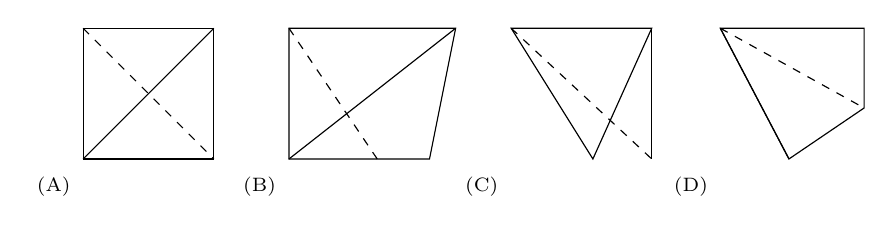
\begin{tikzpicture}[font=\scriptsize, line width=0.42pt, scale=0.83]
  % A
  \begin{scope}
    \node at (-0.45,-0.42) {(A)};
    \draw (0,0)--(2,0)--(2,2)--(0,2)--cycle;
    \draw (0,0)--(2,2);
    \draw[dashed] (0,2)--(2,0);
  \end{scope}
  % B
  \begin{scope}[xshift=3.15cm]
    \node at (-0.45,-0.42) {(B)};
    \draw (0,0)--(2.15,0)--(2.55,2)--(0,2)--cycle;
    \draw (0,0)--(2.55,2);
    \draw[dashed] (0,2)--(1.35,0);
  \end{scope}
  % C
  \begin{scope}[xshift=6.55cm]
    \node at (-0.45,-0.42) {(C)};
    \draw (0,2)--(2.15,2)--(1.25,0)--cycle;
    \draw (2.15,2)--(2.15,0);
    \draw[dashed] (0,2)--(2.15,0);
  \end{scope}
  % D
  \begin{scope}[xshift=9.75cm]
    \node at (-0.45,-0.42) {(D)};
    \draw (0,2)--(2.20,2)--(2.20,0.78)--(1.05,0)--cycle;
    \draw (0,2)--(1.05,0);
    \draw[dashed] (0,2)--(2.20,0.78);
  \end{scope}
\end{tikzpicture}
\end{center}
\nopagebreak[4]
\Needspace{4\baselineskip}
\textbf{解析}

向 $zOx$ 平面投影后，四顶点成为正方形的四个顶点。连接 $(0,0,0)$ 与 $(1,0,1)$ 的棱在前方为实线，连接 $(1,1,0)$ 与 $(0,1,1)$ 的棱被遮挡为虚线，故选 A。

\gkanswer{答案：A}

\end{answer}
\begin{answer}
\gksolhead{10}{}

\textbf{题目}：

设抛物线 $C:y^2=4x$ 的焦点为 $F$，直线 $l$ 过 $F$ 且与 $C$ 交于 $A,B$ 两点，若 $|AF|=3|BF|$，则 $l$ 的方程为\mbox{（　　）}

（A）$y=x-1$ 或 $y=-x+1$　　（B）$y=\dfrac{\sqrt3}{3}(x-1)$ 或 $y=-\dfrac{\sqrt3}{3}(x-1)$

（C）$y=\sqrt3(x-1)$ 或 $y=-\sqrt3(x-1)$　　（D）$y=\dfrac{\sqrt2}{2}(x-1)$ 或 $y=-\dfrac{\sqrt2}{2}(x-1)$

\Needspace{4\baselineskip}
\textbf{解析}

\Needspace{5\baselineskip}
抛物线参数式可取 $(t^2,2t)$，其到焦点的距离为 $t^2+1$。过焦点的弦两端参数满足 $t_1t_2=-1$；由距离比得 $t_1^2=3$。直线斜率为

\nopagebreak[4]
\[\frac{2t_1}{t_1^2-1}=\pm\sqrt3,\]

故选 C。

\gkanswer{答案：C}

\end{answer}
\begin{answer}
\gksolhead{11}{}

\textbf{题目}：

已知函数 $f(x)=x^3+ax^2+bx+c$，下列结论中错误的是\mbox{（　　）}

（A）$\exists x_0\in\mathbb R,\ f(x_0)=0$

（B）函数 $y=f(x)$ 的图象是中心对称图形

（C）若 $x_0$ 是 $f(x)$ 的极小值点，则 $f(x)$ 在区间 $(-\infty,x_0)$ 单调递减

（D）若 $x_0$ 是 $f(x)$ 的极值点，则 $f'(x_0)=0$

\Needspace{4\baselineskip}
\textbf{解析}

三次函数图象总有一个对称中心，且因连续并趋向于相反无穷必有实根，A、B 正确；极值点可在另一个极值点右侧，极小值点左边不必全程递减，故 C 错误。可导函数在内点极值处导数为零，D 正确，选 C。

\gkanswer{答案：C}

\end{answer}
\begin{answer}
\gksolhead{12}{}

\textbf{题目}：

若存在正数 $x$ 使 $2^x(x-a)<1$ 成立，则 $a$ 的取值范围是\mbox{（　　）}

（A）$(-\infty,+\infty)$　　（B）$(-2,+\infty)$　　（C）$(0,+\infty)$　　（D）$(-1,+\infty)$

\Needspace{4\baselineskip}
\textbf{解析}

令 $h(x)=2^x(x-a)$。当 $a>-1$ 时，$x\to0^+$ 有 $h(x)\to-a<1$，故可取充分小的正数 $x$。反之，若 $a\leqslant-1$，则 $x-a\geqslant x+1$，而 $2^x(x+1)>1$，不可能成立。故选 D。

\gkanswer{答案：D}

\end{answer}
\gkpart{二、填空题}

\begin{answer}
\gksolhead{13}{}

\textbf{题目}：

从 $1,2,3,4,5$ 中任意取出两个不同的数，其和为 $5$ 的概率是\gkblank{}。

\Needspace{4\baselineskip}
\textbf{解析}

从五数任取两数共有 $\binom52=10$ 种，和为 $5$ 的为 $\{1,4\}$、$\{2,3\}$ 两种，概率为 $1/5$。

\gkanswer{答案：$\dfrac15$}

\end{answer}
\begin{answer}
\gksolhead{14}{}

\textbf{题目}：

已知正方形 $ABCD$ 的边长为 $2$，$E$ 为 $CD$ 的中点，则 $\overrightarrow{AE}\cdot\overrightarrow{BD}=$\gkblank{}。

\Needspace{4\baselineskip}
\textbf{解析}

\Needspace{5\baselineskip}
取 $A=(0,0),B=(2,0),D=(0,2)$，则 $E=(1,2)$，所以

\nopagebreak[4]
\[\overrightarrow{AE}\cdot\overrightarrow{BD}=(1,2)\cdot(-2,2)=2.\]

\gkanswer{答案：$2$}

\end{answer}
\begin{answer}
\gksolhead{15}{}

\textbf{题目}：

已知正四棱锥 $O-ABCD$ 的体积为 $\dfrac{3\sqrt2}{2}$，底面边长为 $\sqrt3$，则以 $O$ 为球心，$OA$ 为半径的球的表面积为\gkblank{}。

\Needspace{4\baselineskip}
\textbf{解析}

\Needspace{5\baselineskip}
底面积为 $3$，故棱锥高为 $3\sqrt2/2$。底面中心到顶点距离平方为 $3/2$，从而

\nopagebreak[4]
\[OA^2=\left(\frac{3\sqrt2}{2}\right)^2+\frac32=6.\]

球表面积为 $4\pi OA^2=24\pi$。

\gkanswer{答案：$24\pi$}

\end{answer}
\begin{answer}
\gksolhead{16}{}

\textbf{题目}：

函数 $y=\cos(2x+\varphi)\ (-\pi\leqslant\varphi<\pi)$ 的图象向右平移 $\dfrac\pi2$ 个单位后，与函数 $y=\sin\left(2x+\dfrac\pi3\right)$ 的图象重合，则 $\varphi=$\gkblank{}。

\Needspace{4\baselineskip}
\textbf{解析}

\Needspace{5\baselineskip}
右移后函数为 $\cos(2x+\varphi-\pi)$，而

\nopagebreak[4]
\[\sin\left(2x+\frac\pi3\right)=\cos\left(2x-\frac\pi6\right).\]

故 $\varphi-\pi\equiv-\pi/6\pmod {2\pi}$。由 $-\pi\leqslant\varphi<\pi$，得 $\varphi=5\pi/6$。

\gkanswer{答案：$\dfrac{5\pi}{6}$}

\end{answer}
\gkpart{三、解答题}

\begin{answer}
\gksolhead{17}{}

\textbf{题目}：

已知等差数列 $\{a_n\}$ 的公差不为零，$a_1=25$，且 $a_1,a_{11},a_{13}$ 成等比数列。

(1) 求 $\{a_n\}$ 的通项公式；

(2) 求 $a_1+a_4+a_7+\cdots+a_{3n-2}$。

\Needspace{4\baselineskip}
\textbf{解析}

\gksubpart{(1) 求通项}

\Needspace{5\baselineskip}
设公差为 $d$。等比条件给出

\nopagebreak[4]
\[(25+10d)^2=25(25+12d),\]

由 $d\ne0$ 得 $d=-2$，从而 $a_n=25-2(n-1)=27-2n$。

\gksubpart{(2) 求和}

\Needspace{5\baselineskip}
$a_1,a_4,\ldots,a_{3n-2}$ 是首项 $25$、公差 $-6$ 的等差数列，故所求和为

\nopagebreak[4]
\[\frac n2[50-6(n-1)]=n(28-3n).\]

\gkanswer{答案（1）：$a_n=27-2n$}

\gkanswer{答案（2）：$n(28-3n)$}

\end{answer}
\begin{answer}
\gksolhead{18}{}

\textbf{题目}：

如图，直三棱柱 $ABC-A_1B_1C_1$ 中，$D,E$ 分别是 $AB,BB_1$ 的中点。
\nopagebreak[4]
\begin{center}% 2013 全国卷Ⅱ文科第 18 题：直三棱柱 ABC-A_1B_1C_1，D、E 为给定中点。
\begin{tikzpicture}[font=\footnotesize, line width=0.45pt]
  \coordinate (A) at (0,0);
  \coordinate (B) at (1.05,-1.05);
  \coordinate (C) at (4.10,0);
  \coordinate (A1) at (0,3.60);
  \coordinate (B1) at (2.05,1.85);
  \coordinate (C1) at (4.10,3.60);
  \coordinate (D) at ($(A)!0.5!(B)$);
  \coordinate (E) at ($(B)!0.5!(B1)$);
  \draw (A)--(A1)--(C1)--(C)--cycle;
  \draw (A1)--(B1)--(C1);
  \draw (B)--(B1);
  \draw (A1)--(D)--(C);
  \draw (A1)--(E)--(C);
  \draw[dashed] (A)--(B)--(C) (D)--(E) (A1)--(C);
  \node[below left] at (A) {$A$};
  \node[below] at (B) {$B$};
  \node[below right] at (C) {$C$};
  \node[above left] at (A1) {$A_1$};
  \node[above] at (B1) {$B_1$};
  \node[above right] at (C1) {$C_1$};
  \node[below left] at (D) {$D$};
  \node[left] at (E) {$E$};
\end{tikzpicture}
\end{center}
\nopagebreak[4]
(1) 证明：$BC_1\parallel$ 平面 $A_1CD$；

(2) 设 $AA_1=AC=CB=2$，$AB=2\sqrt2$，求三棱锥 $C-A_1DE$ 的体积。

<!-- 固定源 PDF 第 1 页（印刷页 831）至此。 -->

\Needspace{4\baselineskip}
\textbf{解析}

\gksubpart{(1) 证明平行}

\Needspace{5\baselineskip}
令 $\boldsymbol b=\overrightarrow{AB}$、$\boldsymbol c=\overrightarrow{AC}$、$\boldsymbol u=\overrightarrow{AA_1}$。则

\nopagebreak[4]
\[\overrightarrow{BC_1}=\boldsymbol c+\boldsymbol u-\boldsymbol b=(\boldsymbol c-\boldsymbol u)-2\left(\frac{\boldsymbol b}{2}-\boldsymbol u\right).\]

右端两向量分别平行于 $A_1C$、$A_1D$，故 $BC_1\parallel$ 平面 $A_1CD$。

\gksubpart{(2) 求体积}

\Needspace{5\baselineskip}
取 $D$ 为原点，令 $A=(-\sqrt2,0,0)$、$B=(\sqrt2,0,0)$、$C=(0,\sqrt2,0)$，直棱方向为 $z$ 轴，则 $A_1=(-\sqrt2,0,2)$、$E=(\sqrt2,0,1)$。于是

\nopagebreak[4]
\[V_{C-A_1DE}=\frac16\left|\det\begin{pmatrix}0&-\sqrt2&\sqrt2\\ \sqrt2&0&0\\0&2&1\end{pmatrix}\right|=1.\]

\gkanswer{答案（1）：见解析版}

\gkanswer{答案（2）：$1$}

\end{answer}
\begin{answer}
\gksolhead{19}{}

\textbf{题目}：

经销商经销某种农产品，在一个销售季度内，每售出 $1\ \mathrm t$ 该产品获利润 $500$ 元，未售出的产品，每 $1\ \mathrm t$ 亏损 $300$ 元。根据历史资料，得到销售季度内市场需求量的频率分布直方图，如图所示。经销商为下一个销售季度购进了 $130\ \mathrm t$ 该农产品。以 $X$（单位：$\mathrm t$，$100\leqslant X\leqslant150$）表示下一个销售季度内的市场需求量，$T$（单位：元）表示下一个销售季度内经销该农产品的利润。
\nopagebreak[4]
\begin{center}% 2013 全国卷Ⅱ文科第 19 题：频率分布直方图。
\begin{tikzpicture}[font=\footnotesize, >=Stealth, line width=0.42pt, x=0.18cm, y=105cm]
  \draw[->] (-12,0)--(58,0) node[right,align=center] {市场需求量};
  \draw[->] (-10,0)--(-10,0.038) node[above,align=center] {频率\\组距};
  % 坐标轴在 0 与 100 之间的截断符号。
  \draw (-7.8,0.0007)--(-7.0,-0.0007)--(-6.2,0.0007)--(-5.4,-0.0007)--(-4.6,0.0007);
  \draw[dashed] (-10,0.010)--(0,0.010); \node[left,xshift=-1mm] at (-10,0.010) {0.010};
  \draw[dashed] (-10,0.015)--(40,0.015); \node[left,xshift=-1mm] at (-10,0.015) {0.015};
  \draw[dashed] (-10,0.020)--(10,0.020); \node[left,xshift=-1mm] at (-10,0.020) {0.020};
  \draw[dashed] (-10,0.025)--(30,0.025); \node[left,xshift=-1mm] at (-10,0.025) {0.025};
  \draw[dashed] (-10,0.030)--(20,0.030); \node[left,xshift=-1mm] at (-10,0.030) {0.030};
  \draw (0,0) rectangle (10,0.010);
  \draw (10,0) rectangle (20,0.020);
  \draw (20,0) rectangle (30,0.030);
  \draw (30,0) rectangle (40,0.025);
  \draw (40,0) rectangle (50,0.015);
  \node[below] at (-10,0) {$0$};
  \foreach \x/\lab in {0/100,10/110,20/120,30/130,40/140,50/150}
    \node[below] at (\x,0) {\lab};
\end{tikzpicture}
\end{center}
\nopagebreak[4]
(1) 将 $T$ 表示为 $X$ 的函数；

(2) 根据直方图估计利润 $T$ 不少于 $57000$ 元的概率。

\Needspace{4\baselineskip}
\textbf{解析}

\gksubpart{(1) 表示利润}

当 $100\leqslant X\leqslant130$ 时，售出 $X$ 吨、余下 $130-X$ 吨，故 $T=500X-300(130-X)=800X-39000$；当 $X>130$ 时全部售完，$T=65000$。

\gksubpart{(2) 估计概率}

\Needspace{5\baselineskip}
$T\geqslant57000$ 等价于 $X\geqslant120$。直方图中 $[120,130)$、$[130,140)$、$[140,150]$ 的面积之和为

\nopagebreak[4]
\[10(0.030+0.025+0.015)=0.70.\]

\gkanswer{答案（1）：$T=\begin{cases}800X-39000,&100\leqslant X\leqslant130,\\65000,&130<X\leqslant150.\end{cases}$}

\gkanswer{答案（2）：$0.70$}

\end{answer}
\begin{answer}
\gksolhead{20}{}

\textbf{题目}：

在平面直角坐标系 $xOy$ 中，已知圆 $P$ 在 $x$ 轴上截得线段长为 $2\sqrt2$，在 $y$ 轴上截得线段长为 $2\sqrt3$。

(1) 求圆心 $P$ 的轨迹方程；

(2) 若 $P$ 点到直线 $y=x$ 的距离为 $\dfrac{\sqrt2}{2}$，求圆 $P$ 的方程。

\Needspace{4\baselineskip}
\textbf{解析}

\gksubpart{(1) 求轨迹}

\Needspace{5\baselineskip}
设圆心为 $(x,y)$、半径为 $r$。两条弦长条件分别给出

\nopagebreak[4]
\[r^2-y^2=2,\qquad r^2-x^2=3.\]

相减得 $y^2-x^2=1$。

\gksubpart{(2) 求圆方程}

点到 $y=x$ 的距离条件为 $|x-y|=1$。联立 $y^2-x^2=1$，得圆心为 $(0,1)$ 或 $(0,-1)$；再由 $r^2-y^2=2$ 得 $r^2=3$，从而得到两圆方程。

\gkanswer{答案（1）：$y^2-x^2=1$}

\gkanswer{答案（2）：$x^2+(y-1)^2=3$ 或 $x^2+(y+1)^2=3$}

\end{answer}
\begin{answer}
\gksolhead{21}{}

\textbf{题目}：

已知函数 $f(x)=x^2e^{-x}$。

(1) 求 $f(x)$ 的极小值和极大值；

(2) 当曲线 $y=f(x)$ 的切线 $l$ 的斜率为负数时，求 $l$ 在 $x$ 轴上截距的取值范围。

\Needspace{4\baselineskip}
\textbf{解析}

\gksubpart{(1) 求极值}

\nopagebreak[4]
\[f'(x)=e^{-x}x(2-x).\]

函数在 $(-\infty,0)$、$(2,+\infty)$ 上递减，在 $(0,2)$ 上递增，故极小值为 $f(0)=0$，极大值为 $f(2)=4/e^2$。

\gksubpart{(2) 求截距范围}

\Needspace{5\baselineskip}
在 $x=t$ 处的切线斜率为负时，$t\in(-\infty,0)\cup(2,+\infty)$。其 $x$ 轴截距为

\nopagebreak[4]
\[g(t)=t-\frac{f(t)}{f'(t)}=t+1+\frac2{t-2}.\]

$g$ 在 $(-\infty,0)$ 上的值域为 $(-\infty,0)$；在 $(2,+\infty)$ 上于 $t=2+\sqrt2$ 取最小值 $3+2\sqrt2$，故得所求并集。

\gkanswer{答案（1）：极小值为 $0$，极大值为 $\dfrac4{e^2}$。}

\gkanswer{答案（2）：$(-\infty,0)\cup[3+2\sqrt2,+\infty)$。}

\end{answer}
\begin{answer}
\gksolhead{22}{}

\textbf{题目}：

如图，$CD$ 为 $\triangle ABC$ 外接圆的切线，$AB$ 的延长线交直线 $CD$ 于点 $D$，$E,F$ 分别为弦 $AB$ 与弦 $AC$ 上的点，且 $BC\cdot AE=DC\cdot AF$，$B,E,F,C$ 四点共圆。
\nopagebreak[4]
\begin{center}% 2013 全国卷Ⅱ文科第 22 题：外接圆、切线及过 B,E,F,C 的圆。
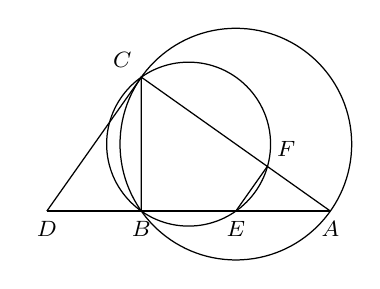
\begin{tikzpicture}[font=\footnotesize, line width=0.45pt]
  \coordinate (B) at (0,0);
  \coordinate (E) at (1.20,0);
  \coordinate (A) at (2.40,0);
  \coordinate (D) at (-1.20,0);
  \coordinate (C) at (0,1.70);
  \coordinate (F) at (1.60,0.567);
  \coordinate (O) at (1.20,0.85);
  \coordinate (o) at (0.60,0.85);
  \draw (O) circle[radius=1.471];
  \draw (o) circle[radius=1.041];
  \draw (D)--(A);
  \draw (D)--(C);
  \draw (B)--(C)--(A);
  \draw (E)--(F);
  \node[below] at (D) {$D$};
  \node[below] at (B) {$B$};
  \node[below] at (E) {$E$};
  \node[below] at (A) {$A$};
  \node[above left] at (C) {$C$};
  \node[above right] at (F) {$F$};
\end{tikzpicture}
\end{center}
\nopagebreak[4]
(1) 证明：$CA$ 是 $\triangle ABC$ 外接圆的直径；

(2) 若 $DB=BE=EA$，求过 $B,E,F,C$ 四点的圆的面积与 $\triangle ABC$ 外接圆面积的比值。

\Needspace{4\baselineskip}
\textbf{解析}

\gksubpart{(1) 证明直径}

记 $BC=a,CA=b,AB=c$。由四点 $B,E,F,C$ 共圆，点 $A$ 的幂给出 $AC\cdot AF=AB\cdot AE$；再与 $BC\cdot AE=DC\cdot AF$ 联立，得 $ab=c\cdot DC$。

\Needspace{5\baselineskip}
切线—割线定理与切线分点的相似关系给出

\nopagebreak[4]
\[DC=\frac{abc}{b^2-a^2}.\]

故 $b^2-a^2=c^2$，即 $b^2=a^2+c^2$。于是 $\angle ABC=90^\circ$，所以 $CA$ 为外接圆直径。

\gksubpart{(2) 求面积比}

设 $DB=BE=EA=t$。则 $AB=2t$，由上问及切线分点关系得 $CA^2:CB^2=3:1$，故 $CB=\sqrt2t$、$CA=\sqrt6t$。又由已知乘积关系得 $AF=\sqrt6t/3$。

\Needspace{5\baselineskip}
取 $B=(0,0),E=(t,0),A=(2t,0),C=(0,\sqrt2t)$，则 $F=(4t/3,\sqrt2t/3)$。过 $B,E,C$ 的圆半径为 $\sqrt3t/2$，而 $CA$ 为外接圆直径，外接圆半径为 $\sqrt6t/2$。面积比为

\nopagebreak[4]
\[\frac{\pi(\sqrt3t/2)^2}{\pi(\sqrt6t/2)^2}=\frac12.\]

\gkanswer{答案（1）：见解析版}

\gkanswer{答案（2）：$\dfrac12$}

\end{answer}
\begin{answer}
\gksolhead{23}{}

\textbf{题目}：

已知动点 $P,Q$ 都在曲线 $C:\begin{cases}x=2\cos t,\\y=2\sin t,\end{cases}\ (t$ 为参数$)$ 上，对应参数分别为 $t=\alpha$ 与 $t=2\alpha\ (0<\alpha<2\pi)$，$M$ 为 $PQ$ 的中点。

(1) 求 $M$ 的轨迹的参数方程；

(2) 将 $M$ 到坐标原点的距离 $d$ 表示为 $\alpha$ 的函数，并判断 $M$ 的轨迹是否经过坐标原点。

\Needspace{4\baselineskip}
\textbf{解析}

\gksubpart{(1) 求参数方程}

\Needspace{5\baselineskip}
两端点坐标取平均，得

\nopagebreak[4]
\[\begin{cases}x=\cos\alpha+\cos2\alpha,\\y=\sin\alpha+\sin2\alpha,\end{cases}\qquad0<\alpha<2\pi.\]

\gksubpart{(2) 判断是否过原点}

\nopagebreak[4]
\[d^2=(\cos\alpha+\cos2\alpha)^2+(\sin\alpha+\sin2\alpha)^2=2+2\cos\alpha,\]

故 $d=2|\cos(\alpha/2)|$。当 $\alpha=\pi$ 时 $d=0$，所以轨迹经过原点。

\gkanswer{答案（1）：$\begin{cases}x=\cos\alpha+\cos2\alpha,\\y=\sin\alpha+\sin2\alpha,\end{cases}\quad0<\alpha<2\pi$。}

\gkanswer{答案（2）：$d=2\left|\cos\dfrac\alpha2\right|$；轨迹经过坐标原点（$\alpha=\pi$）。}

\end{answer}
\begin{answer}
\gksolhead{24}{}

\textbf{题目}：

设 $a,b,c$ 均为正数，且 $a+b+c=1$，证明：

(1) $ab+bc+ca\leqslant\dfrac13$；

(2) $\dfrac{a^2}{b}+\dfrac{b^2}{c}+\dfrac{c^2}{a}\geqslant1$。

\Needspace{4\baselineskip}
\textbf{解析}

\gksubpart{(1) 证明第一式}

由 $(a+b+c)^2\geqslant3(ab+bc+ca)$，结合 $a+b+c=1$，即得 $ab+bc+ca\leqslant1/3$。

\gksubpart{(2) 证明第二式}

\Needspace{5\baselineskip}
由柯西不等式

\nopagebreak[4]
\[\frac{a^2}{b}+\frac{b^2}{c}+\frac{c^2}{a}\geqslant\frac{(a+b+c)^2}{a+b+c}=1,\]

结论成立。

\gkanswer{答案（1）：见解析版}

\gkanswer{答案（2）：见解析版}

\end{answer}